%!TEX root = ../thesis.tex

\chapter{Grundlagen}

Im Folgenden werden Grundlagen erläutert, die als Basis des Projekts sowie zum Verständnis der in Kapitel \ref{chap:frameworks} beschriebenen Technologieauswahl erforderlich sind.


\section{Native Entwicklung}

Bei der Entwicklung nativer Applikationen wird der Programmcode speziell für eine Zielplattform mit dem entsprechendem \ac{SDK} der Plattform entwickelt.
Die App ist damit an die Plattform gebunden. Apps für Apples iOS werden in Swift oder Objective-C entwickelt und nutzen \emph{UIKit} als Framework für die visuelle Darstellung.
Android Apps werden typischerweise in Java implementiert und nutzen das Android Framework als Systemschnittstelle und für die Entwicklung des \ac{UI}.
Nativ entwickelte Apps werden als Binärdatei compiliert, über den jeweiligen Appstore verteilt und auf das Gerät installiert \cite{Heitkoetter2013}.

\vspace{0.3cm}
\textbf{Desktop Nativ}
\begin{itemize}
\item macOS (Swift, ObjectiveC, Java)
\item Linux (C++, C\#, Java)
\item Windows (C++, C\#, VisualBasic, Java)
\end{itemize}
\vspace{0.3cm}

\textbf{Mobil Nativ}
\begin{itemize}
\item iOS (Swift, ObjectiveC)
\item Android (Java)
\end{itemize}
\vspace{0.3cm}

\section{Mobile cross-plattform Entwicklung}

Im Vergleich zum Ansatz der nativen Entwicklung bieten diverse plattformunabhängige Entwicklungsansätze die Möglichkeit, eine Codebasis zu entwickeln,
die auf diversen Plattformen ausgeführt werden kann \cite{Heitkoetter2013}.
Hierbei muss zwischen browserbasierten Web-Apps (Cordova, Phonegap) und cross-kompilierten Applikationen (Xamarin, Titanium, FireMonkey) unterschieden werden
\cite{Xamar84:online}.

\subsection{Cross-kompilierte Apps am Beispiel von Xamarin}

Xamarin Entwickler können den in C\# geschriebenen Code für die Plattformen iOS, Windows Mobile und Android kompilieren.
Der resultierende Code läuft dabei nativ auf den jeweiligen Geräten.
Die Xamarin Entwickler versprechen, dass alles was in Swift, Objective-C und
Java möglich ist, auch mit C\# und Xamarin umgesetzt werden kann \cite{projectxamarin}.

\begin{figure}[ht]
 \centering
 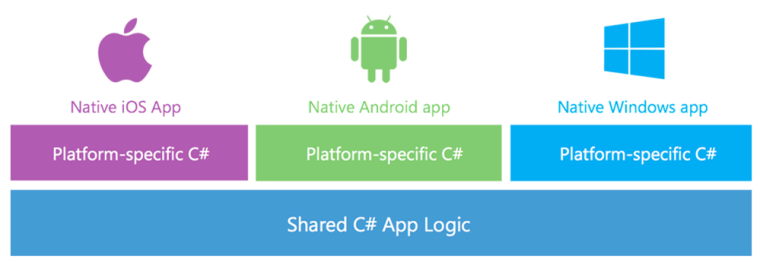
\includegraphics[width=0.8\linewidth]{kapitel2/csharp_xamarin.png}
 \caption{Xamarin Plattformen \cite{7Reas20:online}}
\end{figure}
\vspace{1cm}

\noindent
Xamarin stößt bezüglich \ac{UI} schnell an seine Grenzen. Das \ac{UI} Layer muss aufgrund von Kompatibilitätsproblemen und fehlender Features des Xamarin Framework
für jede Plattform separat entwickelt werden. Dies funktioniert, wenn eine App entsprechend der \ac{CI} der Plattform umgesetzt werden soll und sich die \ac{UI} so weit unterscheidet,
dass Abstraktionen und komponentenbasierte Entwicklung vernachlässibar sind. Es ist jedoch fragwürdig ob sich das Framework als ``cross-platform development software'' bezeichnen darf,
wenn ein Großteil der Implementierung, zumindest bei plattform-universellem Appdesign, nach wie vor redundant vorgenommen werden muss \cite{7Reas20:online}.

\begin{figure}[ht]
 \centering
 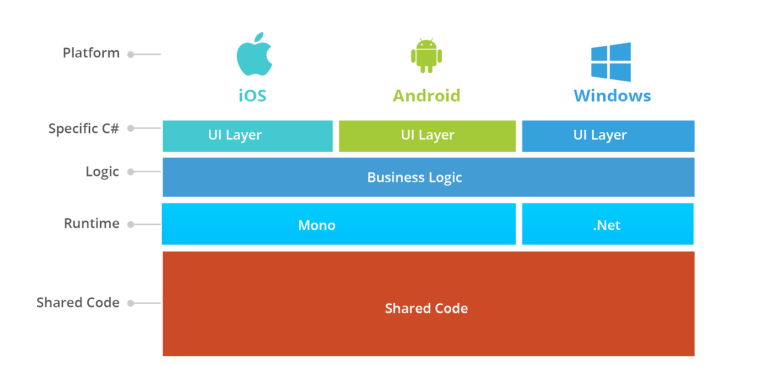
\includegraphics[width=0.8\linewidth]{kapitel2/xamarin_ui_blocker.png}
 \caption{Xamarin Layer \cite{7Reas20:online}}
\end{figure}

\newpage


\subsection{Web-Apps}

Cordova ist ein Framework von Adobe Systems um mobile plattformunabhängige Anwendungen mithilfe von Webtechnologien zu entwickeln.
\ac{HTML}, \ac{CSS} und JavaScript werden genutzt um Produkte für iOS, Android, Ubuntu, Blackberry OS, Firefox OS und Windows Phone zu generieren \cite{Cordo26:online}.
Der Code wird, im Vergleich zu mit Xamarin entwickelten Apps, nicht für verschiedene Plattformen kompiliert,
sondern wird in einer nativen Webview ausgeführt. Diese Anwendungen werden auch als hybride Apps bezeichnet.
Ionic und Phonegap sind Frameworks, die auf der Cordova Technologie basieren.

Zugriff auf Systemschnittstellen erhalten Entwickler mithilfe von Cordova Plugins. Diese bieten
Interfaces in JavaScript für den Zugriff auf native Systemkomponenten wie zum Beispiel Kamera, GPS, Dateisystem et cetera.
Plugins bestehen daher aus JavaScript und dem Plattform kompatiblen Code,
also beispielsweise Swift/Objective-C für iOS oder Java für Android.
Listing \ref{cordova-camera-example} beinhaltet eine Implementierung der Kamera-Schnittstelle über das Plugin \emph{cordova-plugin-camera}.
Das Kamera-Objekt steht global zur Verfügung um innerhalb der Funktion \emph{getPicture} Callbacks für den Erfolg beziehungsweise den Fehlerfall zu registrieren.

\ac{UI} Entwicklung muss dabei im Vergleich zum Xamarin Framework nicht redundant vorgenommen werden, da Implementierungen der
Ansichten für sämtliche unterstützten Plattformen identisch ausgeliefert werden können.
Da die \ac{UI} mithilfe von \ac{HTML} und \ac{CSS} realisiert wird,
können spezielle Stilregeln dennoch auch plattformspezifisch angewandt werden, um beispielsweise eine App zu entwickeln,
welche den jeweiligen Stilrichtlinien der Plattformen entsprechen soll.

\vspace{0.3cm}
\lstinputlisting[language=Javascript,label=cordova-camera-example,caption=Cordova Kamera Example]{kapitel2/cordova-plugin-example.js}
\vspace{0.3cm}

\newpage
\section{Web Components}
\label{sec:webcomponents}


\subsection{Einführung}

Moderne Webanwendungen bestechen heutzutage meist nicht nur mit ihrem komplexen Design, Komplexität lässt sich auch in der Entwicklung
von Funktionalität nicht vermeiden. Dieses Problem wird noch brisanter, wenn eine Applikation über einen langen Zeitraum hinweg,
womöglich von verschiedenen Entwicklerteams, entwickelt und betreut wird. Mit Blick auf das \ac{DOM} moderner und komplexer Webanwendungen wie Facebook, Ebay oder Amazon
wird schnell klar, dass deren Domstruktur durch inflationäre Nutzung von DIV und SPAN Tags schnell zu Unübersichtlichkeit führt
da die Palette an HTML5 Semantic Tags nicht ausreicht um die Funktionalitätsvielfalt einer modernen Webanwendung zu beschreiben.
Statt aussagekräftige Tags zu verwenden, müssen Klassen und IDs zweckentfremdet werden, um HTML Elemente überhaupt voneinander unterscheiden zu können
\cite{sitepoint-introduction-to-webcomponents}.

\subsection{Komponenten in der Softwarentwicklung}

``Modern applications are increasingly
open in terms of topology,
platform and evolution, and so the
need for a component-oriented
approach to development is even
more acute than in the past [...]  Objects provide an organizational
paradigm for decomposing large
applications into cooperating objects
as well as a reuse paradigm for
composing applications from prepackaged
software components.''
\cite{nierstrasz1992component}

\vspace{0.5cm}

Bereits 1992 sprachen Nierstrasz, Gibbs und Tsichritzis vom Traum der komponentenorientierten Softwareentwicklung.
Dabei soll Software aus vielen Komponenten aufgebaut werden, im Idealfall habe man die Möglichkeit ein
ganzes Set an vorgefertigten Komponenten für die Konstruktion seiner Applikation zu verwenden.
Hierbei soll der Aspekt der Abstraktion und Wiederverwendbarkeit durch Objektorientierung von zentraler Bedeutung sein.

\vspace{0.5cm}
``A software component is a unit of composition with contractually specified interfaces and explicit
context dependencies only. A software component can be deployed independently and is subject to composition
by third parties.''
\cite{Szyperski}
\vspace{0.5cm}

Szyperski definiert eine Komponente als eigenständiges, in sich geschlossenes Modul ohne Deployment
Abhängigkeiten, d.h. Eine Komponente kann ausgeliefert werden, ohne dass andere Elemente der Applikation neu compiliert werden müssen.
Klar definierte Schnittstellen dienen der komponentenübergeifenden Kommunikation und repräsentieren
dabei die Funktionalität der Komponente möglichst transparent.
Komponenten sollen dabei angeboten, sei es komerziell oder gratis,
und von Dritten verwendet werden können.


\subsection{Web Components}

``Web Components are an emerging set of standards from the W3C to describe a way to create encapsulated,
reusable blocks of UI presentation and behavior entirely with client side languages- HTML, JavaScript and CSS.''
\cite[42]{Web-Component-Architecture}
\vspace{0.3cm}

Das \ac{W3C} beschreibt diverse Wege, wie entkoppelte wiederverwendbare UI Elemente, sogenannte \emph{Web Components},
in Kombination von \ac{HTML}, JavaScript und \ac{CSS} geschaffen werden können.
Der Begriff Web Components beinhaltet eine Sammlung von Standards,
welche die bereits genannte Problematik der fehlenden HTML Semantik mit bestehenden Webtechnologien lösen kann.
Web Components funktionieren als wiederverwendbare Web Widgets mit klar definierten Schnittstellen.
Dabei sollen sie im Browser implementiert und ohne externe Bibliotheken nutzbar sein.
Bestehende Web Komponenten sollen ohne zusätzlichen Code funktionsfähig sein. Lediglich durch das Einfügen der Komponente
in das Markup, soll bereits die komponenteninterne Funktionalität zur Verfügung stehen
\cite[42]{Web-Component-Architecture}.
Web Components bauen auf vier Kerntechnologien auf: HTML Imports, HTML Teamplates, Custom Elements und Shadow Dom.

\subsubsection{HTML Imports}
HTML kann per Referenz in HTML Dokumente importiert und damit verwendet werden, siehe Listing \ref{htmlimport}.
Dabei können in dem referenziertem HTML Abhängigkeiten in Form von CSS und JS eingebunden werden,
welche dementsprechend aufgelöst werden.
Sollten mehrere Dokumente mit der selben Abhängigkeit eingebunden werden, wird diese dennoch nur einmalig geladen
\cite{HTMLI44:online}.

\vspace{0.3cm}
\lstinputlisting[language=HTML,label=htmlimport,caption=HTML Imports]{kapitel2/html_import.html}
\vspace{0.3cm}

\subsubsection{HTML Templates}

Das HTML Template-Element ermöglicht Inhalte nicht zur Laufzeit der Website zu rendern,
sondern den Rendervorgang explizit per JavaScript zu steuern. Ressourcen wie Videos und Bilder werden demnach
nicht initial geladen und erzeugen keine unnötige Ladeverzögerung der Applikation.
Inhalte des Template-Tags werden zu Beginn auf Validität geprüft und stehen dann für die Verwendung im Dokument
zur Verfügung.

\subsubsection{Custom HTML Elements}

Durch Custom HTML Elements werden \emph{Web Components} in Applikationen eingebunden.
Eigene HTML Tags und Elemente können definiert werden und beinhalten in Javascript geschriebene Logik sowie CSS Styling.
Ein Custom Element besitzt einen Lifecycle mit diversen Einstiegspunkten, welche für die Entwicklung einer Anwendung genutzt werden können.:

\begin{itemize}
\item createdCallback - Element wird registriert
\item attachedCallback - Element wird in den DOM der Applikation eingefügt
\item detachedCallback - Element wird aus dem DOM entfernt
\item attributeChangedCallback - Attribute werden Elementen hinzugefügt, verändert oder entfernt
\end{itemize}


\subsubsection{Shadow Dom}
Der Shadow Dom ermöglicht Optik und Logik einer Komponente zu kapseln.
Seiteneffekte, bezüglich komponentenübergreifendem Style und Logik, werden verhindert.
Beispielsweise kann das Styling eines Menüs nicht aufgrund gleicher CSS Prefixe den Style des Contents überschreiben,
da dieser in die Navigations-Komponente gekapselt ist und nicht auf die globalen Styles des Dokuments oder anderer Elemente zugreifen kann.
Webapplikationen lassen sich dadurch paketweise organisieren und strukturieren.
\subsubsection{Polyfills}
\begin{figure}[htp]
 \centering
 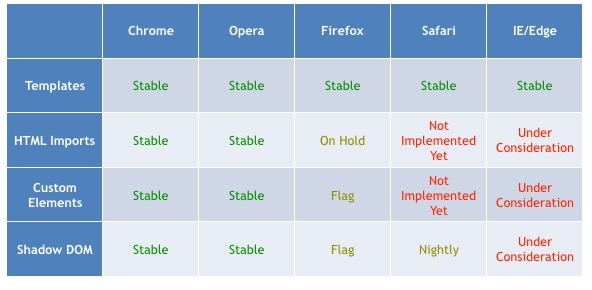
\includegraphics[width=0.7\linewidth]{kapitel2/platform_support.jpg}
 \caption{Plattform Support \cite{WebCo43:online}}
 \label{fig:platform_support}
\end{figure}

\noindent Wie in Abbildung \ref{fig:platform_support} zu erkennen ist, sind elementare Bestandteile, die für die Verwendung von Web Components erforderlich sind, noch nicht in
allen gängigen Browsern nativ verfügbar. Lediglich in Chrome und Opera sind diese vollständig implementiert.
Hier kommen Polyfills ins Spiel. Polyfills implementieren fehlende Browserfeatures und gewährleisten damit beispielsweise nahezu vollständigen
Support von \emph{Web Components} in allen gängigen Browsern. Ein weiteres Beispiel für ein Polyfill ist core-js,
welches die Nutzung der JavaScript Standards \ac{ES5} und \ac{ES6}, auch wenn der Browser diese nicht unterstützt, ermöglicht.



\section{TypeScript}

\subsection{Entwicklung von JavaScript}


JavaScript wurde erstmals 1996 von Brendan Eich in einer Implementierung des Netscape Navigator Browsers eingeführt,
worauf weitere Browser die Syntax und API ähnlich, jedoch nicht identisch nach implementierten.
Daraufhin veröffentlichte die ECMA International einen Standard, welcher die Spezifikationen der neuen Sprache
definieren sollte. Dieser trägt den Namen ECMAScript und ist der offizielle und bekannteste Standard der
Sprache. ActionScript von Macromedia und JScript von Microsoft sind weitere Implementierungen der Browsersprache,
die nicht dem ECMA Standard entsprechen, jedoch darauf aufbauen.

\begin{figure}[hp]
 \centering
 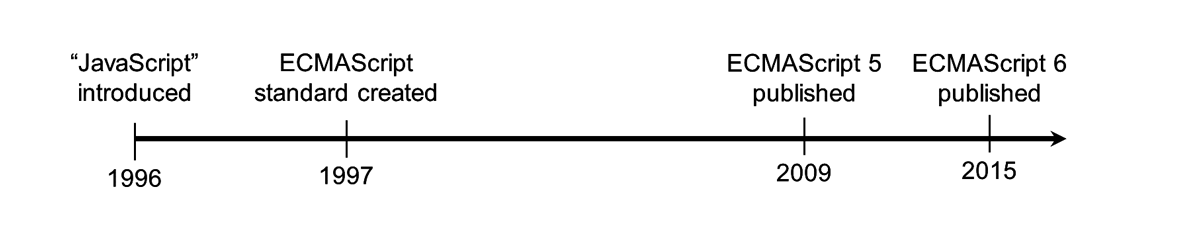
\includegraphics[width=\linewidth]{kapitel2/javascript-timeline.png}
 \caption{Entwicklung von JavaScript \cite[28]{EssentialTS}}
\end{figure}

1997 wurde die erste Version des nun standardisierten ECMAScript veröffentlicht. Ein Jahr später erschien bereits ECMAScript2,
allerdings beinhaltete dieses Update nur kleine Änderungen um einem parallel entstandenen ISO Standard von JavaScript zu implementieren.
Die nächste große Neuerung kam 1999 mit ECMAScript3, in welcher einige innovative Features implementiert wurden.
``[...]regular expressions, better string handling, new control statements, try/catch exception handling, tighter definition of errors, formatting for numeric output and other enhancements.''\cite{js-vs-es}.

Das nächste Update ECMAScript4 war für 2008 geplant und wurde zunächst als Prototyp entwickelt,
es wurde jedoch noch vor dem Release aufgrund eines rückschrittigen Featureset wieder aufgegeben.
Zur selben Zeit etstand Ajax und damit eine völlig neue Art von dynamsichen Webapplikationen,
basierend auf JavaScript.

2009 erschien \ac{ES5} und erhielt kurz darauf vollen Support in nahezu allen verbreiteten Webbrowsern, abgesehen vom Internet Explorer.
Es beinhaltet neue Features wie \ac{JSON} Support und klassische Array Funktionen wie map und forEach.
Durch die Entfernung einiger Features wurde JavaScript in der neuen Version sauberer und stabiler.

\ac{ES6} sollte bereits 2013 veröffentlicht werden, der offizielle Releasetermin wurde
dann allerdings auf den Juni 2015 verschoben und ist bis heute noch nicht ausreichend in allen Browsern implementiert
\cite{js-vs-es}.

\subsection{Allgemein}

TypeScript ist eine von Microsoft entwickelte Programmiersprache.
Die Sprache ist ein Superset von \ac{ES6}, das heißt sie implementiert den JavaScript Standard und ergänzt diesen
durch zusätzliche Features.
TypeScript will ausgereifter, robuster und speziell in großen Projekten eine solidere Alternative gegenüber JavaScript sein \cite[28]{EssentialTS}.
Zusammen mit dem Featureset von \ac{ES6} erhalten Entwickler gegenüber \ac{ES5} die in Abbildung \ref{tsesgraph} dargestellten und im Folgenden beschriebenen Features.

\begin{figure}[ht]
 \centering
 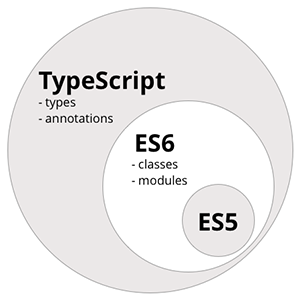
\includegraphics[width=0.4\linewidth]{kapitel2/typescript----es5-es6-typescript-circle-diagram.png}
 \caption{Typescript \cite[152]{ng-Book-2}}
 \label{tsesgraph}
\end{figure}


\subsubsection{statische Typisierung}

Die wohl größte Errungenschaft von TypeScript ist das statische Typsystem.
Typenfehler können bereits zum Zeitpunkt
der Kompilierung bzw. Transpilierung erkannt werden und treten nicht erst zur Laufzeit im Browser auf.
Zudem wird Code in einer TypeScript unterstützenden IDE dank Autovervollständigung
leichter zu schreiben und aussagekräftiger zu lesen \cite[156]{ng-Book-2}.

\subsubsection{Klassen}

Mit ES6 Klassen wurde eine neue Syntax für das prototypische Vererbungsmodell von Javascript entwickelt.
Dabei handelt es sich nicht um die Einführung eines neuen OOP-Modells, sondern lediglich um eine vereinfachte Syntax für Objekte und deren Schnitstellen,
sowie die Realisierung von Abstraktionen, wie sie aus anderen objektorientierten Sprachen, wie C++, Swift oder Java, bereits bekannt sind \cite{js-Klassen}.
Ein Beispiel für eine ES6 Klasse ist in Listing \ref{es6class} implementiert.

\vspace{0.3cm}
\lstinputlisting[language=Java,label=es6class,caption=Klassen in ES6]{kapitel2/class.js}

\subsubsection{Module}

Innerhalb des ES5 Standards gab es keine Möglichkeit Funktionen und Variablen strukturiert in Namensräumen organisieren oder dynamisch laden zu können.
Mit ES6 wurde das fehlende Feature durch den Ex- und Import von Modulen ergänzt. Dadurch ist es einfacher, Programmcode zu organisieren,
da ES6 Module in verschiedene Dateien ausgelagert werden können. Variablen und Funktionen sind von außerhalb nicht sichtbar, es sei denn, sie werden explizit exportiert.
Wie in Listing \ref{jsmodule} dargestellt, lassen sich mittels Export also Schnittstellen für Module definieren, welche daraufhin importiert und verwendet werden können.
In TypeScript lassen sich ganze Klassendefinitionen exportieren.
Dabei ist es möglich, Instanzfunktionen und Instanzvariablen mit dem Keyword private vor dem äußeren Zugriff zu verstecken.
Mit public markierte Funktionen sind dann ebenfalls von außen nutzbar.

\vspace{0.3cm}
\lstinputlisting[language=Javascript,label=jsmodule,caption=Export und Import von Modulen in ES6]{kapitel2/module.js}

\subsection{Decorator}

TypeScript Decorator basieren auf dem Dekorierer Entwurfsmuster (Decorator Design Pattern) um Klassen,
Funktionen, Variablen und Parameter deklarativ um Funktionalität zu erweitern.
Das Konzept der Decorator ist vergleichbar mit dem der Annotations, welches beispielsweise Verwendung in Java, Scala und C\#
finden.
Mithilfe eines Decorators kann eine zentrale Implementierung
mithilfe des @ Symbols und einer nachfolgenden Funktion an Elemente einer Anwendung angebracht werden.
Eine sehr vereinfachte Implementierung eines TypeScript Decorators ist in Listing \ref{decorator-example} dargestellt.

\vspace{0.3cm}
\lstinputlisting[language=Javascript,label=decorator-example,caption=Decorator Beispiel]{kapitel2/decorator-example.ts}
\vspace{0.3cm}


\subsection{Transpilierung}

TypeScript und ES6 bieten Entwicklern eine ganze Reihe von Neuerungen gegenüber den Vorgängerversionen.
Spannende Features bringen jedoch wenig, wenn sie im Standard zwar spezifiziert wurden,
allerdings noch in sehr wenigen Browsern vollständig implementiert sind.
Um TypeScript oder ES6 Code also überhaupt in Produktion nutzen zu können, sollte er auf den ES5 oder ES3
Standard transpiliert werden.
Ein Transpiler ist ein Compiler, welcher Sourcecode nicht in Maschinencode, sondern ebenfalls in Sourcecode,
allerdings einer anderen Sprache oder Sprachversion wandelt \cite{Introduction-to-the-Typescript-Transpiler}.
In der Abbildung \ref{transpile} ist zu sehen, wie TypeScript-Code in funktionsfähigen ES5 Code transpiliert wird.

\begin{figure}[ht]
 \centering
 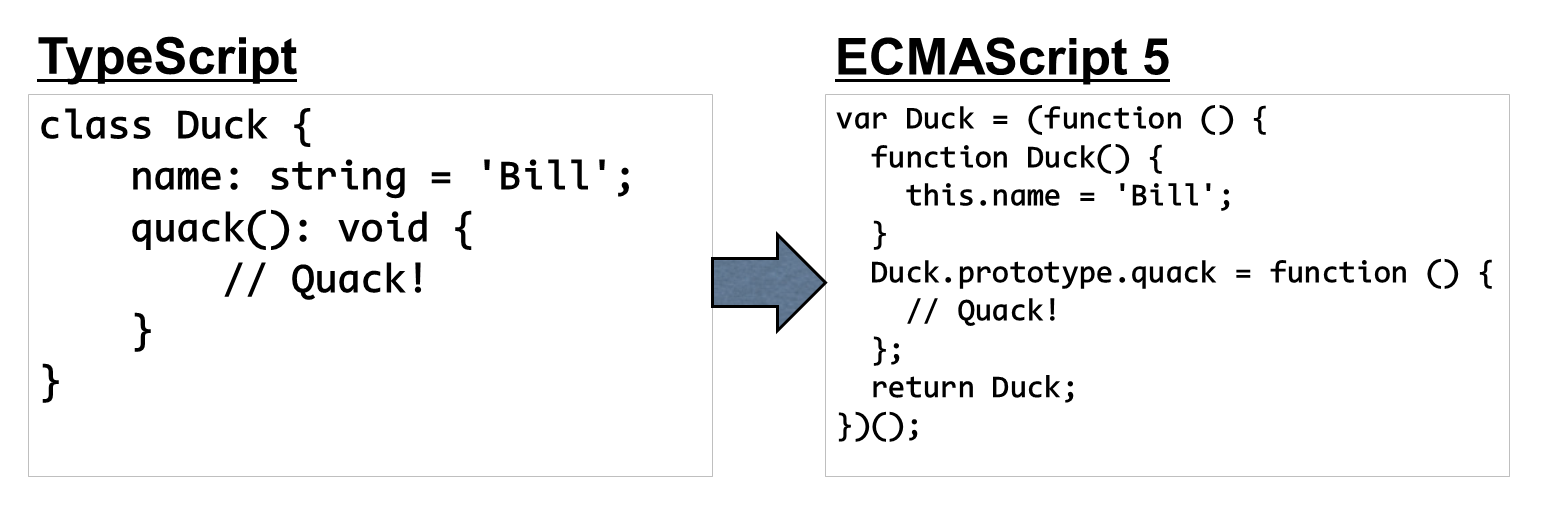
\includegraphics[width=0.8\linewidth]{kapitel2/Introduction-transpiler.png}
 \caption{Transpilierung \cite[27]{ng-Book-2}}
 \label{transpile}
\end{figure}
